\fig{fv:m2:precession}{垂直于角动量的力矩改变方向，不改变角动量大小}{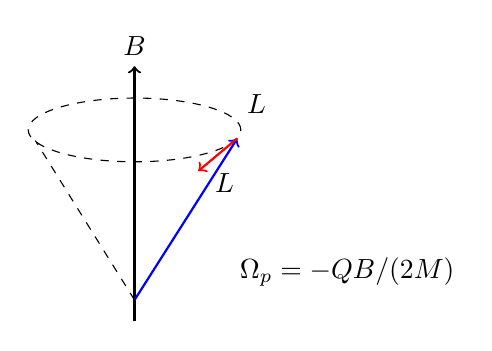
\begin{tikzpicture}[scale=.9]
\draw[->,thick](0,-.3)--(0,3.3)node[above]{$\bm B$};\draw[dashed](0,2.4)ellipse(1.5 and .45);
\draw[->,blue,thick](0,0)--(1.45,2.28);\node[above right]at(1.45,2.5){$\bm L$};\draw[->,red,thick](1.45,2.28)--(.9,1.82);\node[right]at(1,1.65){$\dd\bm L$};
\draw[dashed](0,0)--(-1.4,2.25);\node at(3,.4){$\bm\Omega_p=-Q\bm B/(2M)$};\end{tikzpicture}}
图\ref{fv:m2:precession}中角动量端点沿圆锥绕行，$\bm L\cdot\dot{\bm L}=0$保证其长度不变。由 $\bm m=(Q/2M)\bm L$得到的力矩是 $(Q/2M)\bm L\times\bm B$；要写成进动形式 $\bm\Omega_p\times\bm L$，交换叉积顺序后必须出现负号。图只示意端点的局部切向变化，进动方向还随 $Q$变号。若电荷与质量分布不成比例，或角速度不与角动量平行，就不能直接使用这一单一进动公式。
